\documentclass[12pt,a4paper,final]{article}
\usepackage[left=2.5cm,right=2.5cm,top=2.5cm,bottom=2.5cm]{geometry}

%% IDIOMA
\usepackage[utf8]{inputenc}
\usepackage[portuguese]{babel}

%% TRANSFORMAÇÕES ESTILO CSS
\usepackage{graphicx}

%% ESTÉTICA
\usepackage{enumerate}
\usepackage{booktabs}
\usepackage{amsmath, amsthm, amssymb, amsfonts}
\usepackage{multirow}
\usepackage[hyphens]{url}
\usepackage{subfig}

%% FONTE
\usepackage[T1]{fontenc}
%\usepackage[sc]{mathpazo} % Palatino with smallcaps
\usepackage{mathptmx}
\usepackage{eulervm} % Euler math

%% TIPOGRAFIA
\usepackage{parskip}
\usepackage[activate={true,nocompatibility},final,tracking=true,kerning=true,spacing=true,factor=1100,stretch=10,shrink=10]{microtype}

%% CODIGO
\usepackage{listings}
\usepackage{color}

\definecolor{dkgreen}{rgb}{0,0.6,0}
\definecolor{gray}{rgb}{0.5,0.5,0.5}
\definecolor{mauve}{rgb}{0.58,0,0.82}

\lstset{frame=tb,
  aboveskip=3mm,
  belowskip=3mm,
  showstringspaces=false,
  columns=flexible,
  basicstyle={\small\ttfamily},
  numbers=none,
  numberstyle=\tiny\color{gray},
  keywordstyle=\color{blue},
  commentstyle=\color{dkgreen},
  stringstyle=\color{mauve},
  breaklines=true,
  breakatwhitespace=true,
  tabsize=3
}

\title{Relatório 5 de TCC2/IC}
\author{Ly Sandro Amorim de Campos Salles\\Departamento de Física\\Universidade Federal do Paraná}
\date{\today}

\begin{document}
	\maketitle


  Desde o último encontro foi desenvolvida a estrutura do novo programa de simulações de autômatos celulares. Nela, foi priorizada a modularidade, aumentando a facilidade de corrigir erros e a rapidez em implementar novos autômatos.
  
  \begin{figure}[h]
    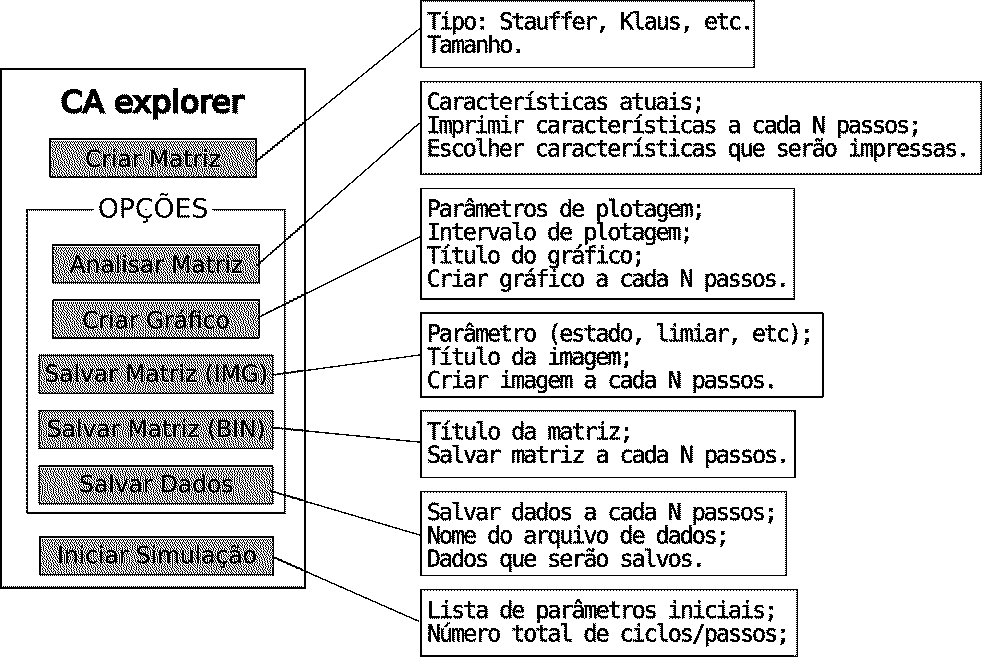
\includegraphics[width=\linewidth]{estruturaCaexplorer.png}
    \caption{Estrutura do novo programa de simulações de autômatos celulares. Apesar de não estar presente na imagem, a opção de incluir a linearização dos dados também estará disponível no menu \texttt{Criar Gráfico}.}
    \label{fig:estruturaCaexplorer}
  \end{figure}

  Para os próximos dias, estas serão as tarefas realizadas:
	\begin{enumerate}
		\item O desenvolvimento do novo programa de simulações de autômatos celulares com base na estrutura acima;
		\item Verificação da sopreposição da curva do potencial de Lennard-Jones no gráfico de afinidade em função de $q$.
		\item Leitura do artigo ``Stochastic Cellular Automata Model for Stock Market Dynamics'' dos autores M. Bartolozzi e A. W. Thomas;
		\item Pesquisa sobre como a volatilidade de mercado influencia na aglomeração dos agentes;
		\item A leitura do Capítulo 4 (``Nonlinear Oscillations and Chaos'') do livro ``Classical Dynamics of Particles and Systems'' dos autores Stephen T. Thornton e Jerry B. Marion.
	\end{enumerate}

\end{document}
